\chapter{The Algorithm} \label{the_algorithm}
	In this chapter we discuss two important object detection algorithms that can classify bubbles in an image and estimate their radii. The first algorithm, which we refer to as \textit{BubbleLow} or simply algorithm \ref{algo:bubbleNet} is optimized to work for small bubble concentration (e.g. figure \ref{fig:aqauarium_result}) whereas algorithm \ref{algo:bubbleCurves}, also referred to as \textit{BubbleCurves} is better suited for bubble images with very high concentrations (figure \ref{fig:aquarium_result_high_conc}).
		
	\section{Motivation}
		We mentioned in section \ref{the_object_detection_problem} that the state of the art object detection algorithms are based on deep learning algorithms such as Faster R-CNN (cite frcnn Leute) and YOLO (Cite yolo Leute). Training these algorithms with our data (simulated and real) did not yield good results. Training a pre-trained R-CNN algorithm (i.e. transfer learning) is not meaningful either because most pre-trained models have large anchors (or rank regions boxes) and are fine tuned to work for real world photographs that contain typical objects such as humans, cars and pets. 
		
		This led us to the conclusion that such algorithms are not well suited for detecting small and dense objects (images with a low bubble concentration are also considered to have dense objects, since they contain several hundred bubble instances per image that are very close to each other). This suspicion was confirmed by (cite Zhenhua Chen et Al.) who also added that these algorithms not only rely on a large amount of training data, but also require the data to be rich in features, which does not apply to our data. 
		
	Interestingly though, scaling down anchors and training an R-CNN algorithm (cite rcnn, Projektpraktikum?) from scratch did perform slightly better, with an IoU@0.5mAP of 68\%. This however, is far from ideal, so developing a different approach was necessary to achieve better results. 
		
		
		
		
	\section{BubbleNet}\label{BubbleNet}
	
	This algorithm detects bubbles in an image with low bubble concentration and estimates their radii. The algorithm extracts candidate signals from images, classifies these signals and then computes a radius from a signal. A vanilla version of the algorithm is described in algorithm \ref{algo:bubbleNet}. Note that the algorithm returns a list of rectangles (i.e. bounding boxes around bubbles) so that we can evaluate its performance. Later on, only bubble radii, i.e. rectangles' widths and depths are needed to construct a bubble spectrum. 
	
			\begin{algorithm}
			\begin{algorithmic}[1]
				\State \textbf{Input} Image with low bubble concentration $G$. 
				\State \textbf{Output} List of rectangles $Rec$, List of depths $Dep$
				\State Obtain local maxima $loc\_max$ in $G$
				\For{Each $lm$ in $loc\_max$}
					\State Extract vertical profile signal $v_p$ with length $L$.
					\If {BubbleNet($v_p$)}
						\State Compute radius $r$ and center $c$ from signal using equation \ref{eq:get_radius}
						\State Compute real radius $r'$ using radius calibration equation \ref{eq:radius_calib}
						\State Compute depth $d$ using equation \ref{eq:dof_calib}
						\State append($Rec$, toBoundingBox($r'$, $c$))
						\State append($Dep$, $d$)
					\EndIf
				\EndFor
			\end{algorithmic}
			
			\caption{BubbleNet}
			\label{algo:bubbleNet}
		\end{algorithm}
	
	\subsection{Radius from Bubble}
	
	A closer inspection of bubbles shows that a bubble can be described well by a vertical cross section going through the middle of the bubble. For instance, figure \ref{fig:bubble_profile} shows that a vertical profile $v_p$ is characterized by a two salient peaks: A bright peak that emerges from total reflection as explained in figure \ref{fig:bubble_physics} as well as a dimmer, yet still visible second peak at a distance $d$ from the first peak. Furthermore, simulation shows that the distance $d$ is proportional to the real bubble radius (figure \ref{fig:peaks_radius_fit}). Note that in figure \ref{fig:peaks_radius_fit} the distance $d$ was computed on rendered images, whereas the radius is a given parameter that is determined before rendering. The step wise increase in $d$ can be explained by sampling, i.e. when the radius increases by an amount smaller than a pixel, $d$ will either not change or increase by exactly 1 pixel.
	
	In order to reach a better precision, we perform a Gaussian fit around the two peaks. Here it is necessary to initialize the fit routine with reasonable values, otherwise both fits would converge towards the same function. So we first smooth the signal with a 1D Gaussian filter, and then determine the absolute maximum $m_1$ within the signal corresponding to the first peak. The second peak corresponds to the highest local maximum $m_2$ that comes right after $m_1$. Finally, we use $arg(m_1)$ and $arg(m_2)$ as initial parameters for a Gaussian fit around the peaks. The final result is given by
	\begin{equation}
		r_{\text{measured}} = \dfrac{| \mu_1 - \mu_2 |}{2}
		\label{eq:get_radius}
	\end{equation}
	for the radius and 
	\begin{equation}
		c_{\text{measured}} =
						 \left( 
							\dfrac{| \mu_1 + \mu_2 |}{2} ,
							 v_{p,y}
						 \right)
	\end{equation}
	for the bubble center 
	where $\mu_1$ and $\mu_2$ are the resulting parameters from the Gaussian fit that correspond the first and second peak respectively. 
	
	From previous considerations it becomes clear that a radius calibration is needed to determine the real radius from the measured radius. This is discussed in sections \ref{sub:radius_setup} and \ref{sub:radius_algorithm}.

		
		\begin{figure}
			\begin{subfigure}[t]{.3\textwidth}
				\centering
				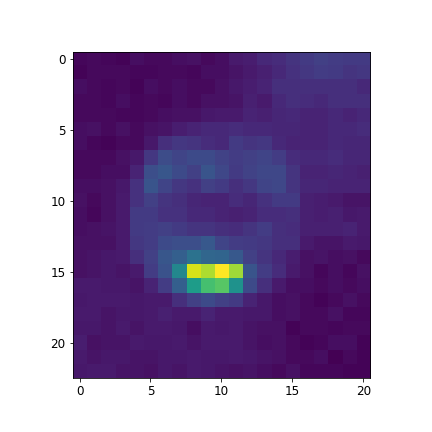
\includegraphics[scale=.5]{images/one_peaks_color.png}
				\caption{Enlarged image of a bubble from a low concentration image. }
			\end{subfigure}\hfill
			\begin{subfigure}[t]{.4\textwidth}
				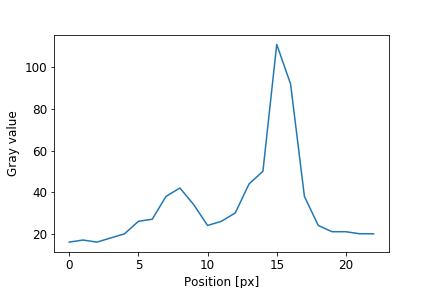
\includegraphics[scale=.5]{graphs/one_peaks_profile.png}
				\caption{Vertical bubble profile. The second peak is much dimmer than the first, but still bright enough to be distinguished from background noise.}
			\end{subfigure}
			\caption{A small air bubble from an image with low bubble concentration.}
			\label{fig:bubble_profile}
		\end{figure}
		
		\begin{figure}
			\centering
			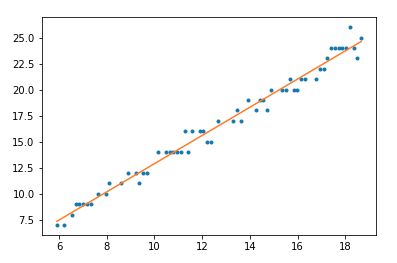
\includegraphics[scale=.7]{graphs/peak_distance_radius_fit.png}
			\caption{Simulated distance between two peaks as a function of bubble radius.}
			\label{fig:peaks_radius_fit}
		\end{figure}
	
	
	
	\subsection{Signal extraction}
		So far, we discussed how we can determine the radius from a given vertical cross section of a bubble. However, the question remains, how do we know the signal corresponds to a bubble in the first place? This is by far more challenging than determining the bubble radius and will be discussed thoroughly in the following sections. 
		
		As we can see from measurement results (section \ref{measurement_result}), extracting local maxima from an image gives good starting points for vertical profile extraction. Starting from a local maximum, we need to go a few pixels downwards $l_{d}$ to cover the whole peak and a certain distance upwards $l_u$ until the second peak is reached. $l_d$ and $l_u$ are hyperparameters that add up to the total signal length $L$. The choice $l_u$ depends on the largest bubble radius that we want to detect. From (cite bubble instrument system) we know that bubbles large enough to loose their spherical shape are very rare and their contribution to gas transfer can be neglected. Also, (cite Leonie) showed that the maximum bubble diameter observed at the Aeolotron facility lies at around 500 $\mu m$ (i.e. 50 pixels). As for $l_d$, a constant value of 4 pixels is good enough to cover the large peak, because the value returned by the fit usually lies within 1 to 2 pixels away from the local maximum. 	
	
		
		\subsection{Signal classification}
		After having extracted a one dimensional signal from a potential bubble, we classify it using a convolutional neural network that we call \textit{BubbleNet}. 

		\subsubsection{BubbleNet architecture}		
		The architecture of our BubbleNet is inspired from (cite Dan Li et al.), where the authors used a 1D convolutional neural network to classify electrocardiogram signals (ECG). The architecture of our CNN is shown in figure \ref{fig:cnn_arch}. We used two convolutional layers with MaxPool layers in between and two dense layers, where the last dense layer is also the output. 
		
		\begin{figure}
			\centering
			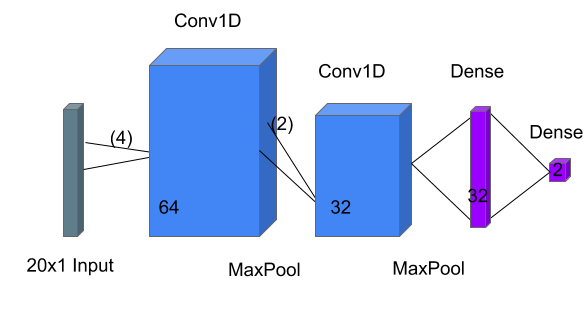
\includegraphics[scale=0.5]{images/cnn_architecture.png}
			\caption{Architecture of BubbleNet. Numbers in parentheses refer to the kernel size. The rest refers to the layer size. }
			\label{fig:cnn_arch}
			
% ########## CNN ##################
%
%		
%	   nb_classes = 2
%    nb_features = 20
%    model = Sequential()
%    model.add(Conv1D(filters=64, kernel_size=4, activation='relu', use_bias=True, input_shape=(nb_features,1)))
%    model.add(MaxPool1D(pool_size=2))
%    model.add(Conv1D(filters=32, kernel_size=2, activation='relu'))
%    model.add(Flatten())
%    model.add(Dense(32))
%    model.add(Activation('relu'))
%    model.add(Dense(nb_classes))
%    model.add(Activation('softmax'))
%		
%
%
%_________________________________________________________________
%Layer (type)                 Output Shape              Param #   
%=======================================================
%conv1d_1 (Conv1D)            (None, 17, 64)            320       
%_________________________________________________________________
%max_pooling1d_1 (MaxPooling1 (None, 8, 64)             0         
%_________________________________________________________________
%conv1d_2 (Conv1D)            (None, 7, 32)             4128      
%_________________________________________________________________
%flatten_1 (Flatten)          (None, 224)               0         
%_________________________________________________________________
%dense_1 (Dense)              (None, 32)                7200      
%_________________________________________________________________
%activation_1 (Activation)    (None, 32)                0         
%_________________________________________________________________
%dense_2 (Dense)              (None, 2)                 66        
%_________________________________________________________________
%activation_2 (Activation)    (None, 2)                 0         
%======================================================
%Total params: 11,714
%Trainable params: 11,714
%Non-trainable params: 0
		\end{figure}
		
	Note that the neural network has a fixed input size of 20 gray values. This means that resizing the vertical profiles is often necessary before passing them to the CNN. We therefore train our CNN with resized inputs in order to make it robust against such preprocessing operations. 
	
	Since the bubble radius is not known prior to vertical profile extraction, we also extract $n$ signals, where 
	\begin{equation}
		r_{min} \leq n \leq L
	\end{equation}
	and then keep the signal with the highest bubble probability. Signals that are classified as background obviously do not get further considerations. $r_{min}$ is the smallest detectable bubble radius and it depends on the magnification factor. For the Aeolotron setup, we have $r_{min} = 90 \mu m$.

		\subsubsection{Training Data}
			The most straightforward approach to generate training data is to annotate images by hand, preferably with an accuracy of no more than 2 pixels. However, this can quickly become very tedious work, especially when hundreds of thousands of images are needed to train a neural network with over $10^{3}$ parameters. Instead, we generated training data as follows:
			\begin{enumerate}
				\item Annotate 300 bubbles only by hand.
				\item Train logistic regression classifier with 300 annotated and 300 simulated images using manually computed features.
				\item Predict 100 000 bubble instances with logistic regression classifier
				\item Use data augmentation to generate a total of 200 000 vertical profiles. 				
				\item Extract 200 000 background (non bubble) images to balance data.
			\end{enumerate}
			
			For step 2, we used following features:
			\begin{itemize}
				\item First peak's gray value $p_1$
				\item Second peak's gray value $p_2$
				\item $p_1/p_2$
				\item Peaks distance $d$
			\end{itemize}
			
			The annotated images are fairly similar in size, lighting conditions and camera settings (Gamma value, gain, exposure time etc..). The reason for that, is because we want to optimize the logistic regression classifier for a high recall, regardless of its precision. So at this stage, we only want to detect as few false positives as possible, even if that means neglecting potential true positives, which in turn lowers the precision. This is obviously not a good approach to classify bubbles, however, our goal at this stage is to merely generate accurately annotated data. After predicting $10^5$ true positive bubble instances from our measurements in step step 3, we processed these images further to generate more data. This included changing the gamma value, resizing (upsampling and downsampling), and vertical flipping. 
			
			Having generated more than $4 \cdot 10^5$, the neural network can now be trained. 
			
			
			
			


			
		\subsubsection{Results}
			
			We first shuffled our data and split it into training (80\%) and testing (20\%). After training for 14 epochs, the testing accuracy converged against 96.8\%, which is a very good result for a binary classifier. 
			
			For validation we used 20 more manually annotated small images, each containing from 10 to 20 bubbles. Figure \ref{fig:bubbleNet_result} illustrates the performance of algorithm \ref{algo:bubbleNet}.  
			The algorithm achieved IoU@0.5mAP = 91.5\% and IoU@0.3mAP = 93\%. Note that this is slightly worse than the classification accuracy result. This is due to the occasionally unprecise radius computation, which gets penalized by the IoU@p-mAP criteria. 
	
			\begin{figure}
				\centering
				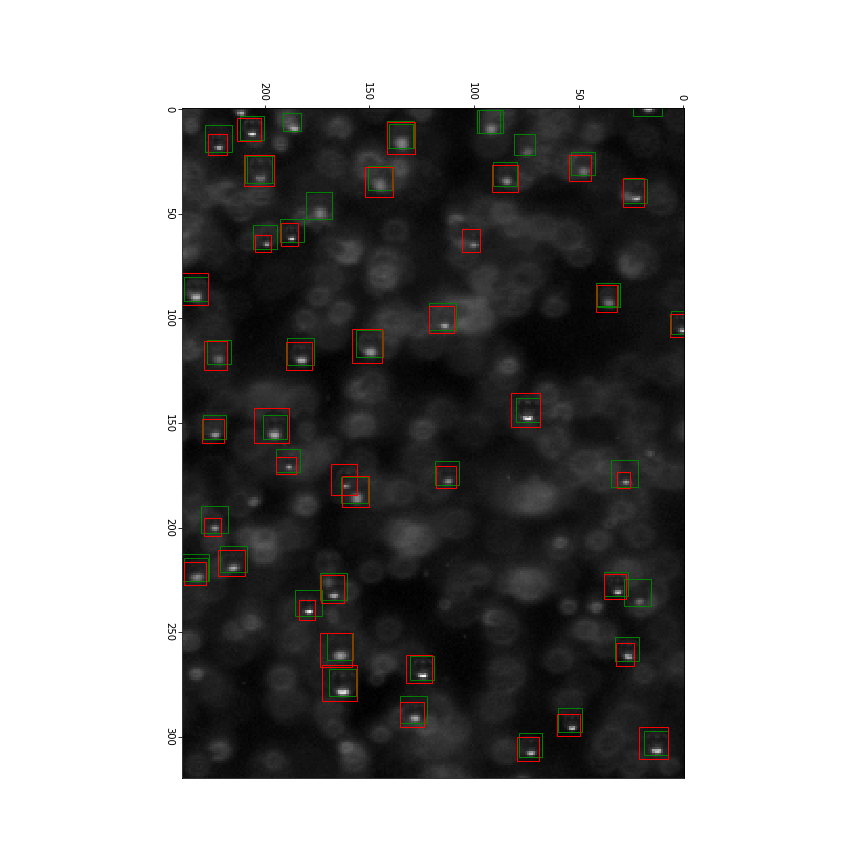
\includegraphics[scale=0.4]{images/bubbleNet_validation_result.png}
				\caption{Testing of algorithm \ref{algo:bubbleNet}. Red: ground truth, green: predicted. Note how in this image, ground truth annotation was not done perfectly, so IoU results were likely slightly underestimated.}
				\label{fig:bubbleNet_result}
			\end{figure}
	
	
	
	
	
	
	\section{BubbleCurves}\label{BubbleCurves}
		This algorithm detects bubbles in images with high bubble concentrations and estimates their radii. In these images, bubble curvatures are much better distinguishable than on low bubble concentrations images. In algorithm \ref{algo:bubbleCurves}, we first pick candidates, classify them and then determine their radii.
	
		\begin{algorithm}
			\begin{algorithmic}[1]
				\State \textbf{Input} Image with a high bubble concentration $G$. 
				\State \textbf{Output} List of rectangles $Rec$, List of depths $Dep$
				\State Obtain local maxima $loc\_max$ in $G$
				\For{Each $lm$ in $loc\_max$}
					\State Extract image window $W$ around $lm$ with size $10 \times 10$.
					\If {RFC($W$)}
						\State get bubble curvature $cur$ 
						\State Compute radius $r$ and center $c$ from $cur$ using a circle fit.
						\State Compute real radius $r'$ using equation \ref{eq:get_radius}
						\State Compute depth $d$ using equation \ref{eq:dof_calib}
						\State append($Rec$, toBoundingBox($r'$, $c$))
						\State append($Dep$, $d$)
					\EndIf
				\EndFor
			\end{algorithmic}
			
			\caption{BubbleCurves}
			\label{algo:bubbleCurves}
		\end{algorithm}
	
	
	
	
	
	
	\subsection{Bubble Classification}\label{bubble_classification}
		In a similar way to algorithm \ref{algo:bubbleNet}, we pick our candidate bubbles based on local maxima in the input image. Then we extract a window with fixed size of $10 \times 10$ pixels around the local maximum. Orientation from structure tensor, the eigenvalues of the structure tensor (see section \ref{radius_from_orientation}) as well as the eigenvalues of the Hessian matrix are used as features to classify bubbles using a random forest classifier. 
		
		The choice of these features is justified as follows. We expect bubbles to show a strong orientation inwards around the local maximum. Therefore we compute the orientation using the structure tensor and expect orientation to be vertical. The eigenvalues of the structure tensor show whether this orientation is significant or not. Finally, with the eigenvalues of the hessian matrix we can determine the curvature around the local maximum, which is expected to be concave. 
		
		As for classification, we chose a random forest classifier (section \ref{rand_forest_class}) because it is well suited for determining thresholds by using decision trees that are particularly robust to inclusion of irrelevant features, which is important when the window size is larger than the considered bubble.
		
		
		
	
	\subsection{Radius from Orientation}\label{radius_from_orientation}
		The idea behind determining the bubble radius is to start from a point on the bubble edge and then "walk" along this edge and keep track of the path. After gathering enough points along this path, we perform a circle fit to determine the bubble's radius and center. 
		
		\subsubsection{Orientation}
		
		Figure \ref{fig:struct_tensor_result} shows the result of applying the structure tensor to a single bubble. We note that orientation arrows describe the orientation as expected around the strongest peak in the image. Since it is only possible to compute the double angle using the structure tensor, the direction of the arrows is not important. In fact, we see a direction flip around the middle of the image. When considering the eigenvalues, we note that both eigenvalues are close to zero around the bubble center and on the upper part of the bubble (figure \ref{subfig:larger_ev} and \ref{subfig:smaller_ev}). This means that orientation around this area is homogeneous (ref theory struct tensor EV interpretation) so results form these area are likely not valid. This is more apparent in figure \ref{fig:struct_tensor_result_2}, where orientation on the upper side is different from the one around the brightest peak in the image. For these reasons, we will only use orientation along the bubble edge up to the middle of the bubble, i.e. where the larger eigenvalue is significantly larger than zero.
		
		\begin{figure}
			\begin{subfigure}[t]{.4\textwidth}
				\centering
				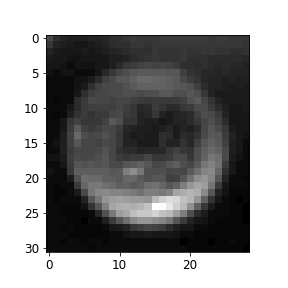
\includegraphics[scale=0.5]{images/struct_tensor_original.png}
				\caption{Original image}		
			\end{subfigure}\hfill
			\begin{subfigure}[t]{.4\textwidth}
				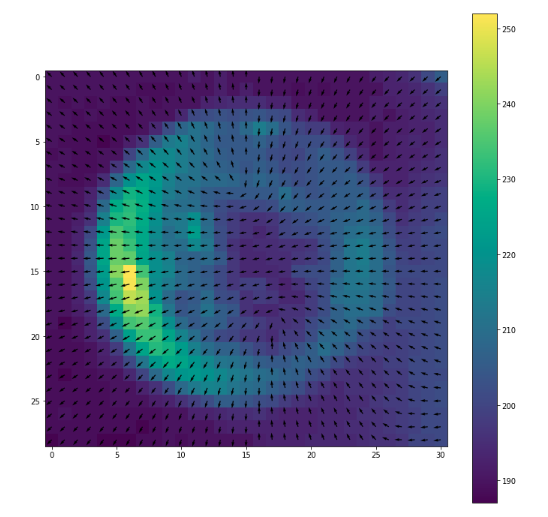
\includegraphics[scale=0.5]{images/struct_tensor_orientation.png}
				\caption{Orientation from structure tensor}		
			\end{subfigure}
			
			\begin{subfigure}[t]{.4\textwidth}
				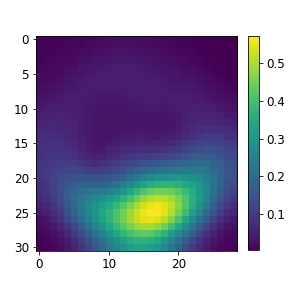
\includegraphics[scale=0.5]{images/larger_ev.png}
				\caption{Larger eigenvalues of the structure tensor}		
				\label{subfig:larger_ev}
			\end{subfigure}\hfill
			\begin{subfigure}[t]{.4\textwidth}
				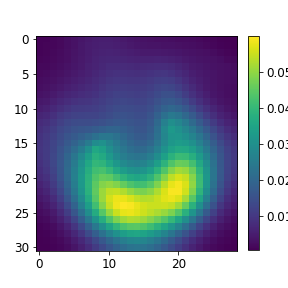
\includegraphics[scale=0.5]{images/smaller_ev.png}
				\caption{Smaller eigenvalues of the structure tensor }
				\label{subfig:smaller_ev}
			\end{subfigure}			
			\caption{Structure tensor eigenvalues and orientation on a single bubble from a high bubble concentration image.}
			\label{fig:struct_tensor_result}
		\end{figure}
		
					
			\begin{SCfigure}
				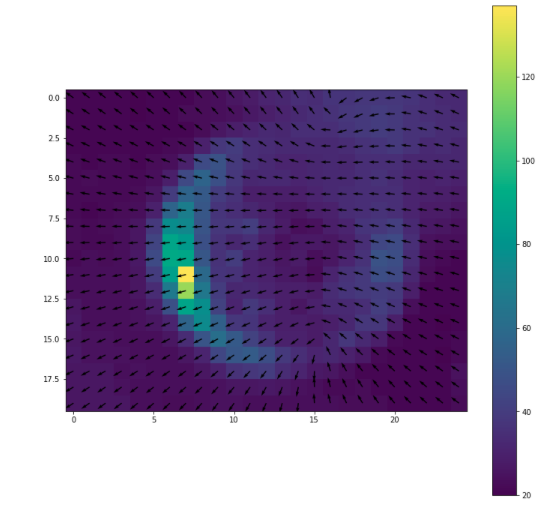
\includegraphics[scale=0.5]{images/struct_tensor_result_2.png}
				\caption{Applying the structure tensor on a slightly smaller and differently lit bubble. Significance of orientation is represented by the arrows' length. Orientation from the left side and the upper part is not meaningful and can't be used.}
				\label{fig:struct_tensor_result_2}
			\end{SCfigure}
	
	
	
	
	
	
	
			\subsubsection{Curve from Orientation}
				Assuming that our starting point is part of the bubble's lower edge, we first get the orientation at the current pixel and then sample points on a line segment along this orientation. The sampling method is taken from (cite max bopp): A square is drawn around each point on the sampling line, and then a weighted average of the gray values within the rectangle is performed, where weights are intersection areas between neighboring pixels and the drawn rectangle. This sampling step is illustrated in figure \ref{fig:subpixel_sampling}
				 After sampling, we perform a Gaussian fit along the fit line, where we initialize the mean with the current position. Next, we add the fit result to our curve and move one step to the right. Figure \ref{fig:curve_from_orientation} summarizes how a bubble curve is extracted using orientation. 
				 
				 \begin{figure}
				 	\centering
				 	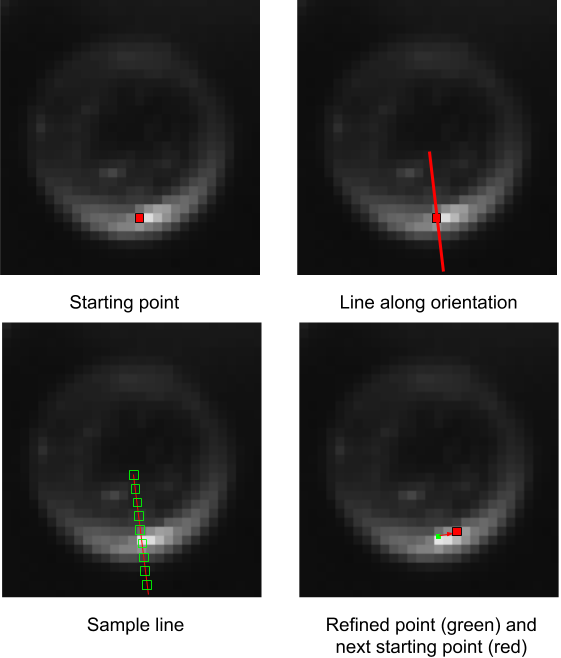
\includegraphics[scale=1]{images/curve_from_orientation.png}
				 	\caption{Extracting curve from bubble using orientation and neighborhood sampling.}
				 	\label{fig:curve_from_orientation}
				 \end{figure}
				 
				 \begin{figure}
				 	\centering
				 	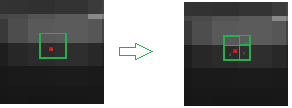
\includegraphics[scale=1]{images/subpixel_sampling.png}
				 	\caption{Gray value sampling along sampling line}
				 	\label{fig:subpixel_sampling}
				 \end{figure}
				 
				
				Finally, we use a least squares fit to find the center $c = (a,b)^T$ and the radius $r$ from the circle equation
				\begin{equation}
					\sqrt{ \left( (x-a)^2 + (y-b)^2 \right)} = r^2
				\end{equation}
				The fit and sampling results are shown in figure \ref{fig:fit_circle_fit_result}
				
				\begin{figure}
				
					\begin{subfigure}[t]{.50\textwidth}
						\centering
						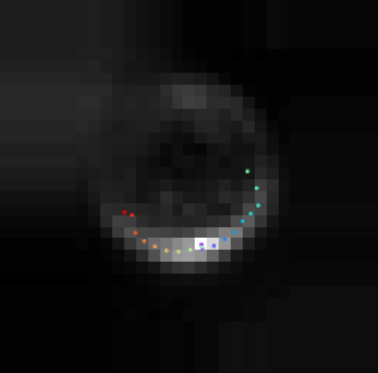
\includegraphics[scale=.8]{images/sampling_result.png}
						\caption{Sampling result. }
					\end{subfigure}					
					\begin{subfigure}[t]{.55\textwidth}
						\centering
						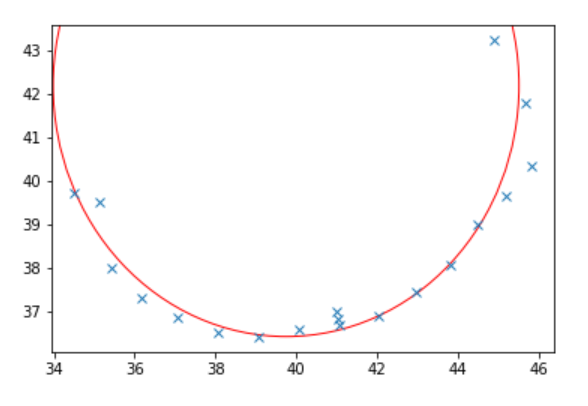
\includegraphics[scale=.7]{graphs/circle_fit.png}
						\caption{Circle fit result.}
					\end{subfigure}
					
					
					\caption{Sampling and fit Note that the circle works well, even though only half a circle is extracted from the bubble at most. }
					\label{fig:fit_circle_fit_result}
				\end{figure}



			\subsubsection{Results}

				\begin{SCfigure}
					\centering
					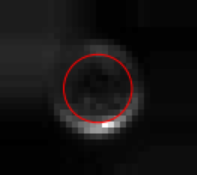
\includegraphics[scale=1.3]{images/bubbleCurve_final_result.png}
					\caption{Final result of algorithm \ref{algo:bubbleCurves} applied to a single bubble}
					\label{fig:final_result}
				\end{SCfigure}
				
				The final result is shown in figure \ref{fig:final_result}. Although the circle matches the bubble's shape well, it is clear that the radius has been underestimated. Similarly to algorithm \ref{algo:bubbleNet}, radius calibration is addressed in section \ref{sub:radius_algorithm}
				
				Using a validation set of 30 small images, each containing 30 to 40 bubbles, this algorithm achieved IoU@0.5mAP = 89.3\%, which is slightly worse than algorithm \ref{algo:bubbleNet}. This is in part due to the high rate of overlap between bubbles, making curvature extraction less precise.. Nevertheless, the algorithm is reliable enough to be usable for bubble detection in high concentration images.
				

	
	
	
	
	\section{Calibration}\label{calibration_algorithm}
		\subsection{Depth of Field}
			Determining the distance between a bubble and the focal plane can be deduced from bubble blurriness. If we consider a vertical profile of the bright lower peak (for both low and high bubble concentration images), we note that the peak's width increases with increasing distance from the focal plane (figure \ref{subfig:peak_profile}). We therefore describe blurriness with the peak's width, given by the sigma parameter of a Gaussian fit around the peak. Theoretically, we would expect a linear dependency between blurriness and distance to focal plane. However, our light source has a certain size that has to be accounted for, which gives bubble peaks a certain minimum width at focus. 
			
			Furthermore, blurriness depends on the radius. For instance, larger bubbles tend to be visible for larger distances from the focal plane (up to 10 centimeters), whereas small bubbles are only visible for no more than 2 centimeters. Figure \ref{subfig:dof_calib_meas} shows measured blurriness (in terms of $\sigma$) as a function of radius and distance from focal plane. 
			
			Therefore, we choose a fourth degree polynomial to describe the blurriness-depth dependency and a linear function to describe the radius dependency. The resulting calibration equation is 
			\begin{equation}
				f(r, d) = b \cdot r + a_1 \cdot d + a_2 \cdot d^2 + c
				\label{eq:dof_calib}				
			\end{equation}
			Where $a_1 =, a_2=, b=, c= $ were used for Aeolotron setup. Figure \ref{subfig:depth_calib_fit_result} shows the two dimensional calibration function alongside the measurements. 
			
			Note that only measurement results up to a certain threshold $\sigma_{th}$ were kept and used for the fit function \ref{eq:dof_calib}. 
			
			
			
			
			\begin{figure}
				\begin{subfigure}[t]{.50\textwidth}
						\centering
						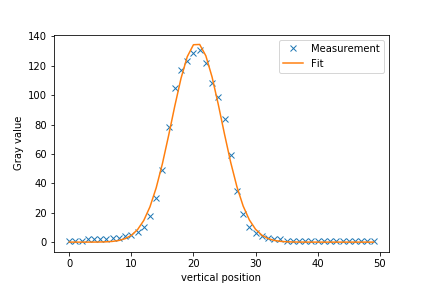
\includegraphics[scale=.4]{graphs/peak_profile_fit.png}
						\caption{Vertical peak profile and Gaussian fit with $\sigma = 4.04$}
						\label{subfig:peak_profile}
					\end{subfigure}\hfill
				\begin{subfigure}[t]{.50\textwidth}
						\centering
						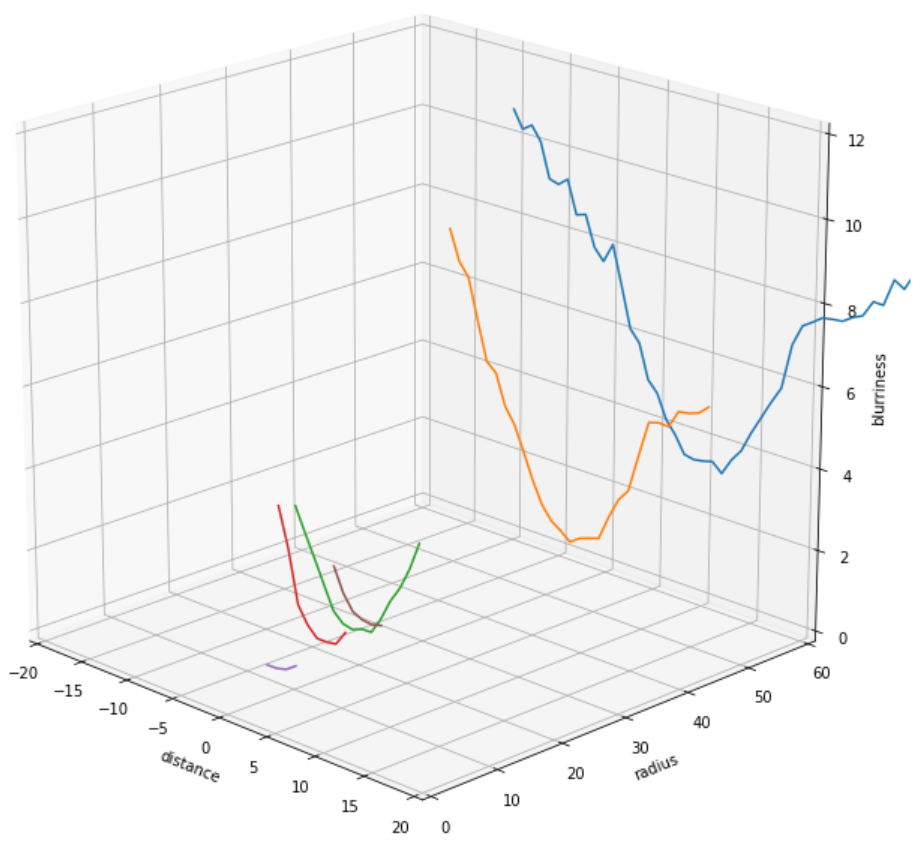
\includegraphics[scale=.4]{images/dof_calibration_measurement.png}
						\caption{ }
						\label{subfig:dof_calib_meas}
					\end{subfigure}				
					
				\begin{subfigure}[t]{.50\textwidth}
						\centering
						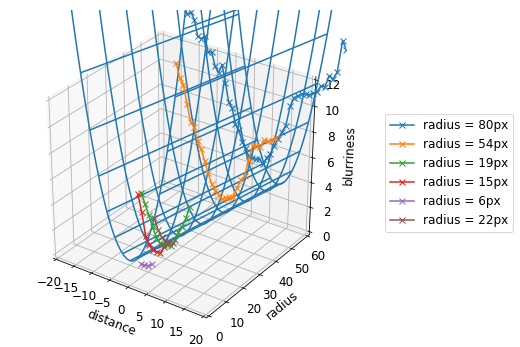
\includegraphics[scale=.4]{images/dof_calibration_fit.png}
						\caption{Sampling result. }
						\label{subfig:depth_calib_fit_result}
					\end{subfigure}								
				
				\caption{Depth calibration}
				\label{fig:depth_calib}
			\end{figure}
			
			
			
			
			
		\subsection{Radius}\label{sub:radius_algorithm}
			The measurement technique developed in this work uses a light source to light up bubbles from below and captures images with a camera placed at $90^\circ$ to the light source. The resulting images are characterized by a lower peak (or bright lower curvature for high concentration bubbles) as discussed in section \ref{measurement_result}. From these images alone, it is not clear whether the observed edge corresponds to the real bubble edge or not. Also, algorithm \ref{algo:bubbleCurves} clearly underestimates the observed radius (figure \ref{fig:final_result}). 
			
			In order to correct for this effect, we performed calibration measurements as described in section \ref{sub:radius_setup}.
			
			We first need to identify back lit bubbles with those lit from below. So we take images with back lit bubbles only, and track a few bubbles of different sizes and depths and compute their radii. From the tracked back lit bubbles, we can roughly estimate the position of the same bubble lit from below. Figure \ref{fig:radius_calib_demo} illustrates the principle behind identifying bubbles from different images. 
			
			\begin{figure}	
				\centering
				\begin{subfigure}[t]{.4\textwidth}
					\centering
					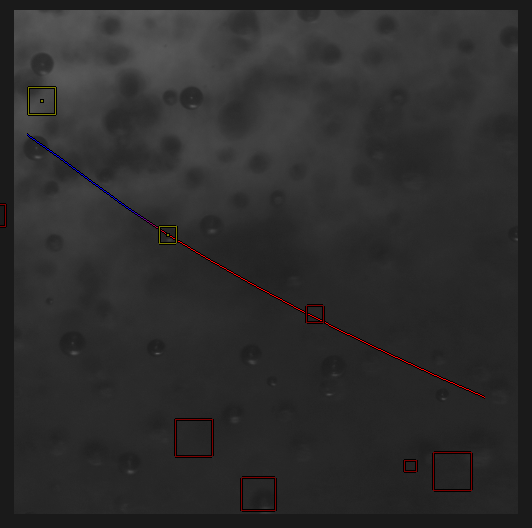
\includegraphics[scale=0.45]{images/tracking_green.png}
					\caption{}
					\label{subfig:green_1}
				\end{subfigure}\hfill
				\begin{subfigure}[t]{.4\textwidth}
					\centering
					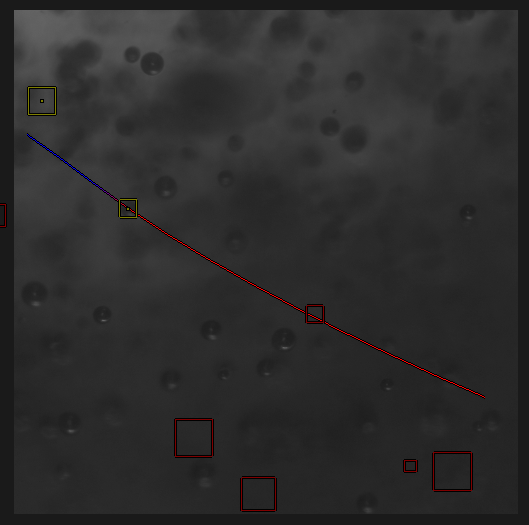
\includegraphics[scale=0.45]{images/tracking_green_2.png}
					\caption{}
					\label{subfig:green_2}
				\end{subfigure}

				\begin{subfigure}[t]{.55\textwidth}
					\centering
					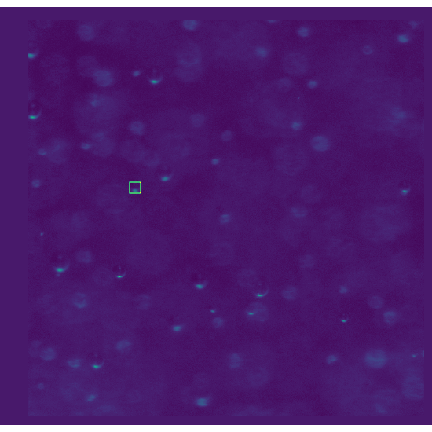
\includegraphics[scale=0.45]{images/tracking_red.png}
					\caption{}
					\label{subfig:red}
				\end{subfigure}
								
					\caption{Identifying a bubble from images with different lighting. Images were acquired at 200 FPS. Image \ref{subfig:red} was taken after \ref{subfig:green_1} and before \ref{subfig:green_2}. Matching bubble in \ref{subfig:red} is marked in red }
					\label{fig:radius_calib_demo}
			\end{figure}
			
			
			Determining the radius of bubbles lit from below is done using algorithm \ref{algo:bubbleNet}. As for the corresponding back lit bubbles, the radius is determined as follows:
			First, we compute the derivative image and then estimate the position of the bubble center using the characteristic bright peak around the bubble center. We then extract several horizontal profiles that go through or are very close to the bubble center. Next, we compute the local maxima from the extracted profiles and apply a Gaussian fit around them in order to determine the local maximum with a subpixel accuracy. The bubble diameter is then given by the distance between the two local maxima that are farthest apart from each other. Figure \ref{fig:green_radius} illustrates the described steps above. 
			
			\begin{figure}
				\centering

				\begin{subfigure}[t]{.4\textwidth}
					\centering
					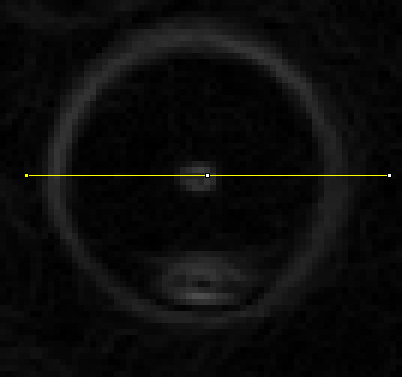
\includegraphics[scale=0.3]{images/green_edges.png}
					\caption{From derivative image we extract horizontal profiles}
				\end{subfigure}\hfill
				\begin{subfigure}[t]{.5\textwidth}
					\centering
					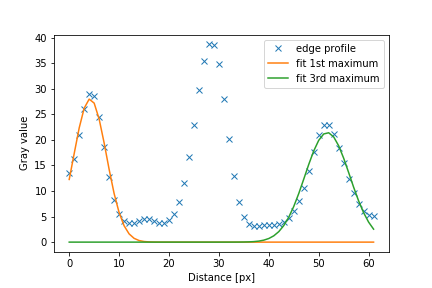
\includegraphics[scale=.6]{graphs/green_radius_demo.png}
					\caption{The distance between the farthest local maxima gives the diameter}
				\end{subfigure}
				
				\caption{Determining the radius of a back lit bubble}								
				\label{fig:green_radius}
			\end{figure}
			
			Figure \ref{fig:radius_calib_result} shows the radius determined by algorithm \ref{algo:bubbleNet} of bubbles lit from below as a function of the radius of back lit bubbles. The error bars are standard deviations, i.e. statistical errors arising from multiple radius computations of the same bubble at different depths and different locations. The resulting radius calibration equation is 
			\begin{equation}
				r' = a \cdot r + b
				\label{eq:radius_calib}
			\end{equation}
			Where $a= 0.95$ and $b=4.54$ were used for the Aeolotron setup. 
			
			\begin{figure}
				\centering
				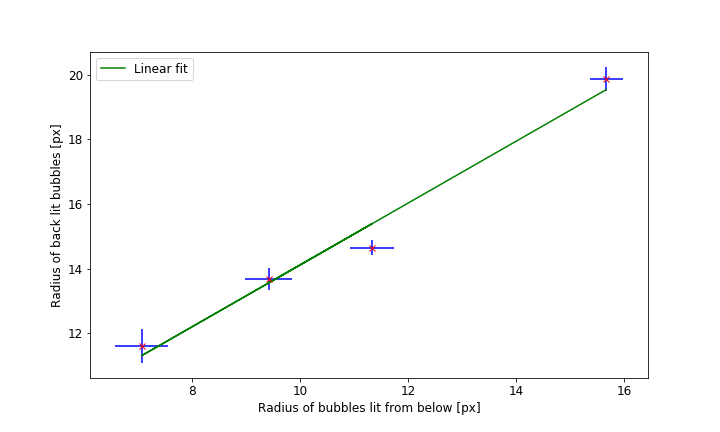
\includegraphics[scale=.6]{graphs/radius_calibration_result.png}
				\caption{Measured radius as a function of real radius.}
				\label{fig:radius_calib_result}
			\end{figure}
			
			
			
			
			
































